\documentclass[crop=True]{standalone}
\usepackage{tikz}
\begin{document}
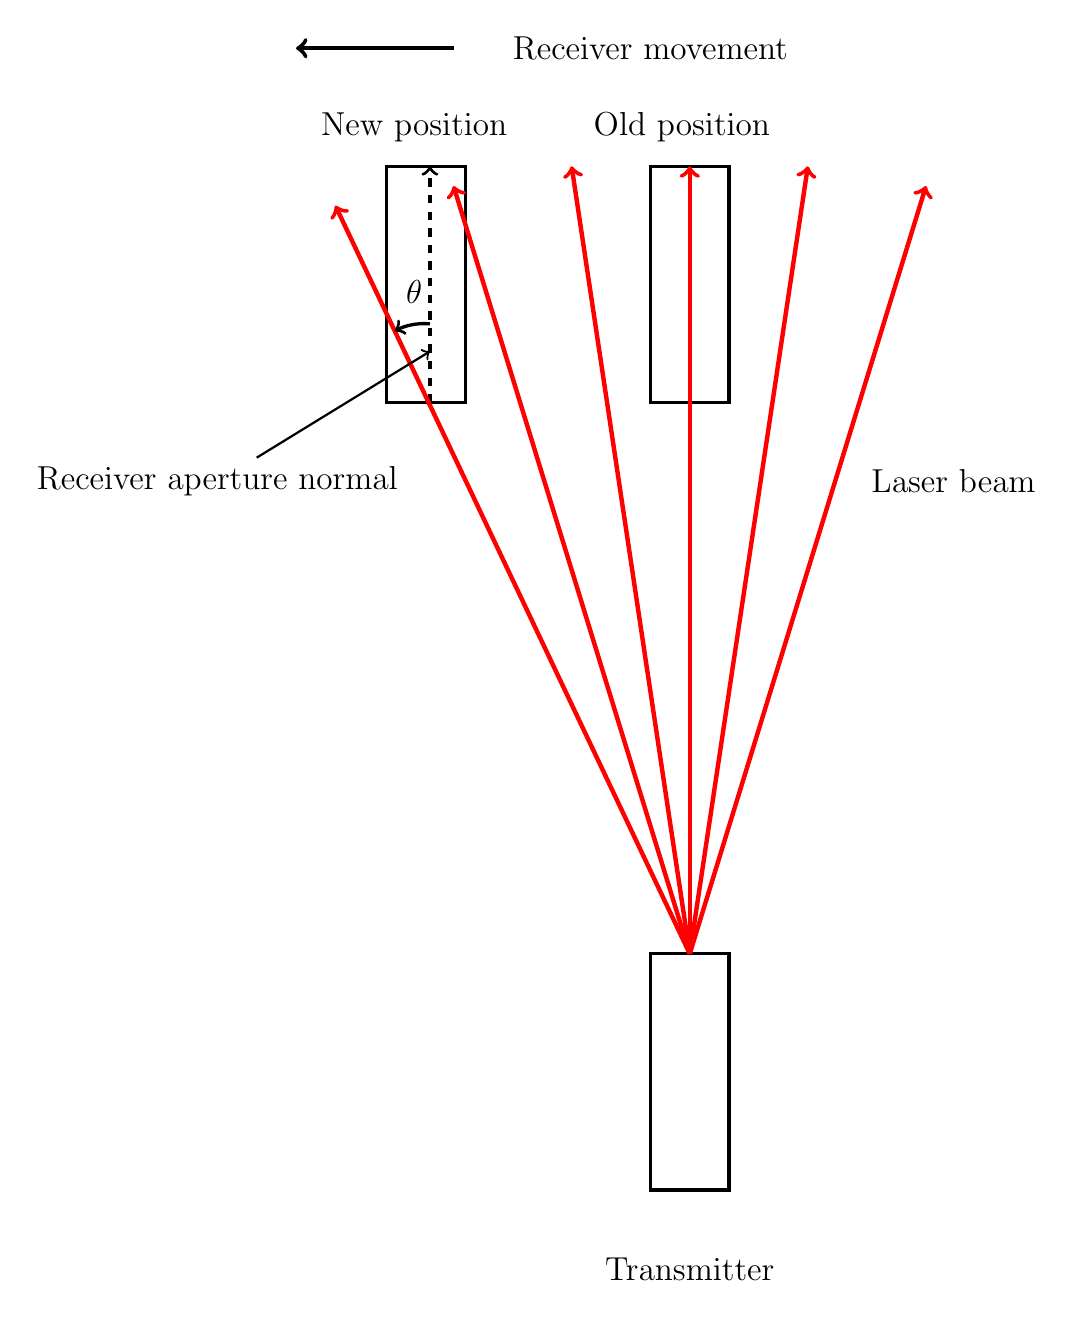
\begin{tikzpicture}



\draw[ very thick] (0,0) rectangle (1, 3);

\draw[ very thick] (-3.35,0) rectangle (-2.35, 3);

\draw[->, very thick, dashed] (-2.8, 0) -- (-2.8, 3);

\draw[ very thick] (0, -10) rectangle (1, -7);

\draw[->, ultra thick, red] (0.5, -7)--(-1, 3);

\draw[->, ultra thick, red] (0.5, -7)--(0.5, 3);


\draw[->, ultra thick, red] (0.5, -7)--(2, 3);

\draw[->, ultra thick, red] (0.5, -7)--(3.5, 2.75);

\draw[->, ultra thick, red] (0.5, -7)--(-2.5, 2.75);

\draw[->, ultra thick, red] (0.5, -7)--(-4, 2.5);

\node at (-3, 1.4) {\large $\theta$};

\draw[very thick, ->] (-2.8,1) arc (85:118:0.8cm);

\node at (0.5, -11){\large Transmitter};

\node at (0, 4.5){\large Receiver movement};

\node at (0.4, 3.5){\large Old position};

\node at (-3, 3.5){\large New position};

\node at (-5.5, -1){\large Receiver aperture normal};

\draw[->, thick] (-5, -0.7)--(-2.8, 0.65);

\draw[->, ultra thick] (-2.5, 4.5)--(-4.5, 4.5);

\node at (3.85, -1){\large Laser beam};


\end{tikzpicture}
\end{document}